% !TEX root = ../../presentation.tex
% Meta: Planung

\newlength{\offset}\setlength{\offset}{0.7cm}
\newlength{\step}\setlength{\step}{1.3cm}

\begin{slide}{Planung}
  \begin{tikzpicture}[thick]
    \tikzset{dot/.style={fill, circle, inner sep=1.3pt}};

    % Timeline
    \draw [|->] (0, 0) -- ++(10.5, 0);

    % Timeline Labels
    \foreach \i/\month in {%
      0/Juni, 1/Juli, 2/August, 3/Sept.,%
      4/Oktober, 5/Nov., 6/Dezember, 7/Januar} {
      \draw ({\i * \step + \offset}, 0.125) -- ++(0, -0.25)
            node [below] {\scriptsize\month};
    }

    % Tasks
    \newcommand{\early}{1}
    \newcommand{\ontime}{2}
    \newcommand{\late}{3}
    \foreach \name/\month/\y/\state in {%
      Architektur/0/1/\ontime,%
      Speichermodell/1/2.75/\late,%
      Instruktionen/2.5/0.5/\early,%
      Assemblierung/3.5/2/\late,%
      Direktiven \& Makros/2/4/\late,%
      Serialisierung/4/1/\ontime,%
      Pseudoinstruktionen/4/3.5/\ontime,%
      {I/O Module}/5/2.75/\late,%
      Dokumentation/6.5/1.5/\ontime%
    } {
      \ifnum\state=1
        \newcommand{\dotcolor}{Green}
        \newcommand{\startslide}{3}
      \else
        \ifnum\state=2
          \newcommand{\dotcolor}{ProcessBlue}
          \newcommand{\startslide}{2}
        \else
          \newcommand{\dotcolor}{Red}
          \newcommand{\startslide}{4}
        \fi
      \fi
      \onslide<\startslide->{
        \path ({\month * \step + \offset}, \y) coordinate [dot, \dotcolor]
              node [above] {\scriptsize\name};
      }
    }

    % Legend
    \onslide<2->{
      \path (8.5, 5.5) coordinate [ProcessBlue, dot] (ontime)
            node [right] {\scriptsize\hspace{0.1cm}Rechtzeitig};
    }

    \onslide<3->{
      \path (ontime)+(0, -0.4) coordinate [Green, dot]
            (early) node [right] {\scriptsize\hspace{0.1cm}Fr\"{u}hzeitig};
    }

    \onslide<4->{
      \path (early)+(0, -0.4) coordinate [Red, dot]
            (late) node [right] {\scriptsize\hspace{0.1cm}Spät};
    }

    % Legend Bounding Box
    \draw [rounded corners=1pt] (ontime)+(-0.3, +0.35) rectangle ++(1.8, -1.1);

  \end{tikzpicture}
\end{slide}

\begin{slide}{Planung}
  \begin{tikzpicture}[thick]
    \tikzset{dot/.style={fill, circle, inner sep=1.3pt}};

    % Timeline
    \draw [|->] (0, 0) -- ++(10.5, 0);

    % Timeline Labels
    \foreach \i/\month in {%
      0/Juni, 1/Juli, 2/August, 3/Sept.,%
      4/Oktober, 5/Nov., 6/Dezember, 7/Januar} {
      \draw ({\i * \step + \offset}, 0.125) -- ++(0, -0.25)
            node [below] {\scriptsize\month};
    }

    % Tasks
    \foreach \name/\planned/\actual/\y in {%
      Speichermodell/1/4/2.75,%
      Assemblierung/3.5/6/2,%
      Direktiven und Makros/2/5/4,%
      {I/O Module}/5/7/2.75,
      Instruktionen/2.5/1/0.5%
    } {
      \ifnum\actual<\planned
        \newcommand{\dotcolor}{Green}
      \else
      \newcommand{\dotcolor}{Red}
      \fi
      \path ({\planned * \step + \offset}, \y)
            coordinate [\dotcolor, dot] (p\name);

      \path ({\actual  * \step + \offset}, \y)
            coordinate [\dotcolor, dot] (a\name);

      \draw [->, dotted, \dotcolor]
            (p\name) -- (a\name) node [above, midway]
            {\color{black}\scriptsize\name};
    }

    % Legend
    \draw (8, 5.85);
  \end{tikzpicture}
\end{slide}

% Einige Gruende hierfuer werden im Team Bericht gegeben und diskutiert

\begin{slide}{Exekution}
  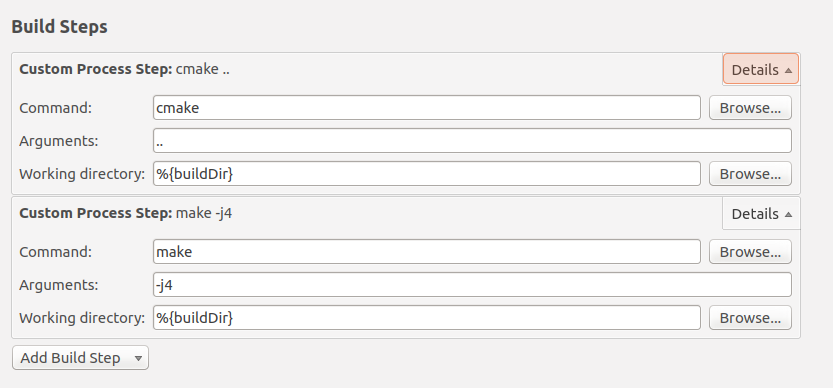
\includegraphics[scale=0.31]{commit-history}
\end{slide}
